\setchapterpreamble[u]{\margintoc}
\chapter{Conclusions}
\label{ch:conclusions}

This chapter aims to summarize the outcomes of this thesis, highlight the most relevant achievements and outline some lines of work that will be pursued next.

\section{Summary of work}

The candidate has been working under a competitive government contract for university professor training with the objective of completing this thesis. Additionally, the doctoral program at University of Granada includes a comprehensive range of lectures and courses which provide formative resources for doctoral candidates. In consequence, the work throughout this period can be categorized into three parts: research, training and teaching.

\subsection{Research activity}

The research developed by the candidate has been already mostly discussed in Chapter~\ref{ch:summary}. The outputs have been multiple and have covered all necessary areas from the study of the state of the art, to developing a new solution to an existing problem and applying it to a specific case.

In summary, during the course of the pre-doctoral stage, the candidate has authored 11 peer-reviewed journal articles, 10 of them being in JCR journals and 8 of those in Q1 within the corresponding knowledge areas. Additionally, the candidate has attended three national AI-focused conferences and two international ones, and has presented works on all of them.

Most of the developed software to perform experimentations has been made available in the popular code repository GitHub for its use to replicate and extend them. Additionally, some of these packages conveniently allow users to apply the models to other datasets, more specifically, Ruta and the autoencoders for complexity reduction including the convolutional version of Slicer. The most relevant source code pieces are described below:

\begin{itemize}
    \item Ruta, software for unsupervised deep architectures (associated to Article~\ref{ch:paper2}). Homepage: \href{https://ruta.software/}{ruta.software}. Source code: \href{https://github.com/fdavidcl/ruta}{github.com/fdavidcl/ruta}.
    \item Autoencoder case studies (associated to Article~\ref{ch:paper5}). Homepage/source code: \href{https://github.com/ari-dasci/S-autoencoder-case-studies}{github.com/fdavidcl/ae-case-studies}.
    \item Reducing complexity (associated to Article~\ref{ch:paper6}). Homepage: \href{https://ari-dasci.github.io/S-reducing-complexity/}{ari-dasci.github.io/S-reducing-complexity}. Source code:\newline \href{https://github.com/ari-dasci/S-reducing-complexity}{github.com/ari-dasci/S-reducing-complexity}.
    \item Convolutional Slicer (associated to \sidecite{charte2021slicer}). Homepage/source code: \href{https://github.com/fdavidcl/slicer-conv}{github.com/fdavidcl/slicer-conv}.
\end{itemize}


\subsection{Formative activity}

% \xr{completar / oficinavirtual está caída -.-}

The different organisms of the University of Granada offer a wide variety of courses, workshops and seminars which help doctoral students complete their training and augment their skills. The candidate has leveraged this as much as time has allowed, having attended to the events detailed in \autoref{ch:formative}.

\begin{table*}[htbp]
    \resizebox{\linewidth}{!}{%
    \begin{tabular}{rp{6cm}p{3.5cm}p{3.5cm}}
        \toprule
        \bfseries Year &\bfseries  Title &\bfseries  Speaker(s) &\bfseries  Organization \\
        \midrule
        2018 & Iniciación a la docencia universitaria para contratados/as predoctorales FPU y FPI & multiple & UGR \\
        2019 & Open Access, Data Management y Data Protection & Pilar Rico,\newline María José Ariza & OPI-UGR, FECYT, Biblioteca UGR \\
        2019 & Workshop de Inteligencia Artificial (Microsoft Azure) & Eduardo Matallanas & Microsoft/Plain Concepts\\
        2020 & Inverse Problems in Image Processing & Mehran Ebrahimi & CITIC-UGR \\
        2020 & ¿Cómo afrontar con éxito una estancia de investigación? & Nicolás Robinson & Vicerrectorado de investigación\\
        2021 & Taller virtual de iniciación a la divulgación & Carlos Centeno,\newline Susana Escudero & DaSCI \\
        2022 & Taller de formación Google Cloud (NLP) & Javier Martínez & Google \\
        2020-22 & DaSCI Online Seminars & multiple & DaSCI \\
        \bottomrule
    \end{tabular}}
    \caption{\label{ch:formative}Relation of courses and seminars the candidate has attended.}
\end{table*}

\subsection{Teaching activity}

The candidate has fulfilled the teaching objectives marked by the FPU regulations: between 3 and 6 ECTS credits a year, totaling at most 18 ECTS credits. More specifically, the amount of credits has been maxed out, achieving the total of 18 credits taught across 4 years.

Taught subjects have belonged to the Computer Science department and to two different disciplines: data structures and models of computation. \autoref{tbl:classes} details the subjects, groups and credits taught each year.

\begin{table}[htbp]
    \resizebox{\linewidth}{!}{
    \begin{tabular}{rllrr}
        \toprule
        \bfseries Year & \bfseries Degree & \bfseries Subject &\bfseries  Groups &\bfseries  ECTS\\
        \midrule
        $2019$ & GII & Estructuras de datos & 1 & $1.5$\\
        $2019$ & GIM & Estructuras de datos & 1 & $1.5$\\
        $2019$ & GII & Modelos de computación & 1 & $3.0$\\
        $2020$ & GII & Estructuras de datos & 2 & $3.0$\\
        $2020$ & GII & Modelos de computación & 1 & $3.0$\\
        $2021$ & GII & Modelos de computación & 2 & $6.0$\\
        \bottomrule
    \end{tabular}}
    \caption[Breakdown of the subjects where the candidate taught practical lectures.]{\label{tbl:classes}Breakdown of the subjects where the candidate taught practical lectures during the doctoral period, detailing the number of groups and the total of ECTS credits. Abbreviations: Grado en Ingeniería Informática (GII), Doble Grado en Ingeniería Informática y Matemáticas (GIM).}
\end{table}



In addition to the mandatory classes, during the course of the thesis, a textbook on machine learning and data science has been published for use as training material \sidecite{mybook}, as well as a 5-video course on linear algebra and dimensionality reduction, including autoencoder networks. The latter, part of a larger machine learning course titled Math-ML, has been created in collaboration with the Andalusian Research Institute in Data Science and Computational Intelligence (DaSCI). The video playlist can be accessed at \href{https://www.youtube.com/playlist?list=PL88MWrW4s4nf-Bc3hccxt3Att8TSS-LBn}{youtube.com/playlist?list=PL88MWrW4s4nf-Bc3hccxt3Att8TSS-LBn}.

% \subsection{Other outcomes}


\subsection{Collaboration with public and private entities}[Collaborations]

The doctoral period also opened opportunities to participate in  collaborations established between the research group and other institutions and companies. The following is a list of these:

\begin{itemize}
    \item Our research group has obtained several state-funded projects which involve deep learning as one of their main lines of work. Their funding allowed the group to build the necessary infrastructure to quickly develop and test models with large amounts of data.
    \item The candidate has collaborated with the Repsol statistics department in optimization of refinery processes. No research outputs are available due to industrial secrecy requirements.
    \item The candidate has participated in a two-year collaboration with the metallurgic company ArcelorMittal, on the topic of semantic segmentation of metallographic iamges with encoder-decoder deep neural networks. A result of this project was the article \sidecite{metallography} co-written by the UGR and ArcelorMittal teams.
    \item A collaboration was also established with the Hospital Universitario San Cecilio in Granada, during which the candidate looked into capsule networks and convolutional networks attempting to solve the problem of detecting the presence of COVID-19-induced lung affection. The results of this study were published in \sidecite{covid}.
\end{itemize}

\section{Achieved objectives}

This section explains how the different objectives posed in Section~\ref{sec:objectives} have been tackled and completed.

\subsection{Didactic resources about autoencoders}[Didactic resources]

Our first objective was tied to the inexistence of a modern, exhaustive and accessible survey on the main tool, the autoencoder. The result was an extensive article (reproduced as Article~\ref{ch:paper1}) that explained every fundamental aspect about these models, as well as provided enough detail about the main variants to be able to select an appropriate one for any given purpose. 

One key contribution of this work was Section~\autoref{p1Sec.HowToChoose}, which attempts to provide advice on which options to choose depending on the problem at hand. This article has achieved more than 100 citations according to Web of Science and more than 200 in Google Scholar, confirming that there was a need for this kind of resource on autoencoders in the research community.

\subsection{Easy-to-use autoencoder implementations}[Implementations]

The main software-related outcome of this thesis has been the R package Ruta (see Article~\ref{ch:paper2}), a library which includes the most relevant autoencoder variants and provides easy-to-use functionalities for beginners, as well as more flexible and detailed options for more experienced users. This software is published at CRAN, a software repository for the R language with strict quality controls.

The Ruta package has totaled more than 15000 downloads just on the official RStudio CRAN mirror, averaging more than 10 downloads per day since its launch. Figure~\ref{fig:rutadl} shows daily downloads of the library according to the RStudio CRAN logs.

\begin{figure*}[htbp]
    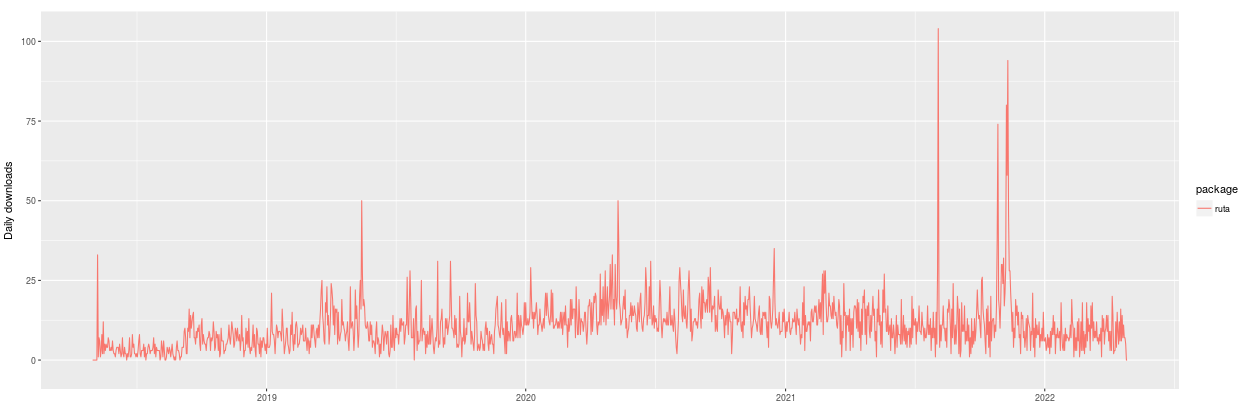
\includegraphics{rutadownloads}
    \caption{\label{fig:rutadl}Per-day downloads of the Ruta package from the RStudio CRAN mirror.}
\end{figure*}

\subsection{Exploration of supervised problems}[Supervised tasks]

The importance of this work, materialized in Article~\ref{ch:paper3}, resides in the fact that it helps connect all the different problem structures that can be encountered in supervised learning, from the simplest to the more general ones. More concretely, \autoref{p3fig.mouttax} visually explains how each problem relates to another by means of generalizations. This can help scientists and practitioners tackle new problem structures by means of known techniques from other problems.

\subsection{Development and application of new autoencoder models}[New models]


The novel contribution developed to satify this objective comprised three new penalty functions that proved to alter the behavior of an autoencoder in a way that was beneficial to undertake a posterior classification task.

The extensive experimentation showed that, out of the three methods considered, the LSSVM-inspired loss worked best and provided significant improvement in classification performance with respect to other feature learners.

% \subsection{Application of newly developed models}

When this model in particular was applied to the image classification problem given by the COVIDGR dataset, results revealed a promising line of work, as several of the selected classifiers improved their performance when learning from the features extracted by the proposed model with respect to the original features.

% \section{Summary of research outcomes}

% This section holds a relation of all public results of the thesis, including the publications that have been reproduced from \autoref{ch:paper1} to \autoref{ch:paper6}, the related software packages and repositories that allow to replicate experimental results, as well as publications arising from collaborations with colleagues and other projects.

% \subsection{Peer-reviewed publications}

% Following are the publications in JCR journals and international conferences associated to the present thesis.

% \subsubsection{Publications in JCR journals}

% The five articles published in journals which are directly linked to the thesis are \sidecite{INFFUS18-AutoencoderTutorial,charte2019ruta,charte2019snapshot,charte2020analysis,charte2021reducing}. Four of them are published in JCR Q1 journals, including an article in IEEE TPAMI which is the highest ranking journal in the area of Computer Science-Artificial Intelligence. The remaining article, published in Progress in Artificial Intelligence, was listed as Q3 in the ESCI (Emerging Sources Citation Index) ranking in 2018. 
% Additionally, two highly related works were presented in international conferences \sidecite{charte2019showcase,charte2021slicer}.



% \begin{itemize}
%     \item \fullcite{}%Charte, D., Charte, F., García, S., del Jesus, M. J., \& Herrera, F. (2018). A practical tutorial on autoencoders for nonlinear feature fusion: Taxonomy, models, software and guidelines. Information Fusion, 44, 78-96.
%     \item Charte, D., Charte, F., García, S., \& Herrera, F. (2019). A snapshot on nonstandard supervised learning problems: taxonomy, relationships, problem transformations and algorithm adaptations. Progress in Artificial Intelligence, 8(1), 1-14.
%     \item Charte, D., Herrera, F., \& Charte, F. (2019). Ruta: Implementations of neural autoencoders in R. Knowledge-Based Systems, 174, 4-8.
%     \item Charte, D., Charte, F., del Jesus, M. J., \& Herrera, F. (2020). An analysis on the use of autoencoders for representation learning: Fundamentals, learning task case studies, explainability and challenges. Neurocomputing, 404, 93-107.
%     \item Charte, D., Charte, F., \& Herrera, F. (2021). Reducing Data Complexity using Autoencoders with Class-informed Loss Functions. IEEE Transactions on Pattern Analysis and Machine Intelligence.
% \end{itemize}

% \subsubsection{Communications in international conferences}


% \begin{itemize}
%     \item Charte, D., Charte, F., del Jesus, M. J., \& Herrera, F. (2019, June). A Showcase of the Use of Autoencoders in Feature Learning Applications. In International Work-Conference on the Interplay Between Natural and Artificial Computation (pp. 412-421). Springer, Cham.
%     \item Charte, D., Sevillano-García, I., Lucena-González, M. J., Martín-Rodríguez, J. L., Charte, F., \& Herrera, F. (2021, September). Slicer: Feature Learning for Class Separability with Least-Squares Support Vector Machine Loss and COVID-19 Chest X-Ray Case Study. In International Conference on Hybrid Artificial Intelligence Systems (pp. 305-315). Springer, Cham.
% \end{itemize}


% \subsection{Collaborations and other related results}

% This section is dedicated to works published during the thesis period where the doctoral candidate participated, as well as talks and dissemination material around the topic of the present thesis.

% \subsubsection{Articles published in collaboration with other researchers with tangential topics to the current thesis}

% Six other JCR articles have been co-authored by the candidate, their topics interleaving with the present thesis but not core to the main objectives \sidecite{mldr,cometa,interplay,covid,complexity,metallography}. 

% \begin{itemize}
%     \item Charte, F., Rivera, A. J., \textbf{Charte, D.}, del Jesus, M. J., \& Herrera, F. (2018). Tips, guidelines and tools for managing multi-label datasets: The mldr.datasets R package and the Cometa data repository. Neurocomputing, 289, 68-85.
%     \item Górriz, J. M., Ramírez, J., Ortíz, A., Martinez-Murcia, F. J., Segovia, F., Suckling, J., \dots \textbf{Charte, D.}, \dots \& Ferrández, J. M. (2020). Artificial intelligence within the interplay between natural and artificial computation: Advances in data science, trends and applications. Neurocomputing, 410, 237-270.
%     \item Tabik, S., Gómez-Ríos, A., Martín-Rodríguez, J. L., Sevillano-García, I., Rey-Area, M., \textbf{Charte, D.}, \dots \& Herrera, F. (2020). COVIDGR dataset and COVID-SDNet methodology for predicting COVID-19 based on chest X-ray images. IEEE Journal of biomedical and health informatics, 24(12), 3595-3605.
%     \item Pascual-Triana, J. D., \textbf{Charte, D.}, Andrés Arroyo, M., Fernández, A., \& Herrera, F. (2021). Revisiting data complexity metrics based on morphology for overlap and imbalance: snapshot, new overlap number of balls metrics and singular problems prospect. Knowledge and Information Systems, 63(7), 1961-1989.
%     \item Luengo, J., Moreno, R., Sevillano, I., \textbf{Charte, D.}, Peláez-Vegas, A., Fernández-Moreno, M., \dots \& Herrera, F. (2022). A tutorial on the segmentation of metallographic images: Taxonomy, new MetalDAM dataset, deep learning-based ensemble model, experimental analysis and challenges. Information Fusion, 78, 232-253.
% \end{itemize}

% \subsubsection{Other conferences and talks}

% The following talks and works were presented in national-level conferences and other events:

% \begin{itemize}
%     \item Charte, D., Charte, F., Herrera, F. (2017). Unsupervised Deep Learning in R with Ruta. Poster presented at \textit{IX Jornadas de Usuarios de R} in Granada.
%     \item Charte, D., Charte, F., García, S., del Jesus, M.J., Herrera, F. (2018). Keywork "A practical tutorial on autoencoders for nonlinear feature fusion" presented at \textit{XVIII Conferencia de la Asociación Española para la Inteligencia Artificial (CAEPIA)} in Granada.
%     \item Charte, D. (2019). Aplicaciones prácticas de las redes neuronales no supervisadas. Talk presented at \textit{esLibre 2019} within track "Informática y matemáticas", in Granada.
%     \item Charte, D. (2020). Autoencoders: An Overview and Applications. Talk presented at \textit{IAA-CSIC Severo Ochoa School on Machine Learning, Big Data, and Deep Learning in Astronomy (SOMACHINE 2020)}.
% \end{itemize}

% \subsubsection{Educational/training material}


% \subsection{Published software}

% Most of the developed software to perform experimentations has been made available in the popular code repository GitHub for its use to replicate and extend them. Additionally, some of these packages conveniently allow users to apply the models to other datasets, more specifically, Ruta and the autoencoders for complexity reduction including the convolutional version of Slicer.

% \begin{itemize}
%     \item Ruta, software for unsupervised deep architectures (associated to \autoref{ch:paper2}). Homepage: \href{https://ruta.software/}{ruta.software}. Source code: \href{https://github.com/fdavidcl/ruta}{github.com/fdavidcl/ruta}.
%     \item autoencoder-showcase (associated to \autoref{ch:paper4}). Homepage/source code: \href{https://github.com/ari-dasci/S-autoencoder-showcase}{github.com/ari-dasci/S-autoencoder-showcase}.
%     \item ae-case-studies (associated to \autoref{ch:paper5}). Homepage/source code: \href{https://github.com/fdavidcl/ae-case-studies}{github.com/fdavidcl/ae-case-studies}.
%     \item Reducing complexity (associated to \autoref{ch:paper6}). Homepage: \href{https://ari-dasci.github.io/S-reducing-complexity/}{ari-dasci.github.io/S-reducing-complexity}. Source code: \href{https://github.com/ari-dasci/S-reducing-complexity}{github.com/ari-dasci/S-reducing-complexity}.
%     \item Convolutional Slicer (associated to \autoref{ch:paper7}). Homepage/source code: \href{https://github.com/fdavidcl/slicer-conv}{github.com/fdavidcl/slicer-conv}.
% \end{itemize}


% \setchapterpreamble[u]{\margintoc}
\section{Future lines of work}
% \label{ch:future}

The developed work has shown to be very promising and opens several possible routes to continue researching. 

\subsection{Promoting other behavior in learned representations}[Other penalties]

As was learned out of the study of autoencoder variants in Article~\ref{ch:paper1} and the new autoencoder models from Article~\ref{ch:paper6}, these models are flexible enough to be able to accept very diverse penalty functions which in turn influence the learned transformations in some way. Relevant uses of this property have been to learn noise-resilient representations, create probability distributions from which to sample new data, and separate points from different classes. 

Leveraging this advantage of autoencoders and taking into account the diversity of supervised problems analyzed in Article~\ref{ch:paper3}, an interesting path of research would be to conceptualize and implement new penalties which incorporate knowledge about the structure of those problems and allow this way to perform feature preprocessing on those tasks, even potentially transformations from one task type to another. For example, one specifically designed autoencoder could merge features from multi-view input samples in order to output just one feature vector, representative of the whole instance. This would effectively reduce multi-view problems to single-view ones.

\subsection{Label separability in multilabel data}[Multilabel separability]

The early work of the candidate, although not fundamental for this thesis, revolved around learning from multilabel data. The previous experience in this specific area would help translate the newly developed solutions in Article~\ref{ch:paper6} from the binary classification scheme to multilabel clasification, as this can be seen as a generalization of the more traditional binary case. 

Approaching label separability, however, is not as straightforward as class separability in binary or multiclass problems, since several labels can co-occur in the same instance. This means that separability is no longer easy to measure: one could compute per-label data complexity measures but that would not give a complete account of how close instances with similar labelsets are. Similarly, for a model to be able to project instances to a feature space better suited for classification, it has to take all labels into account at the same time and produce variables that separate not only individual labels but relevant labelsets.

Multilabel learning being typically a harder problem than multiclass classification, there is a need for better descriptive and preprocessing tools, so a set of complexity measures and new methods for reducing complexity in datasets of this kind would be a notable advancement. Some preliminary work is currently being done by the candidate with this purpose in mind.

\subsection{Synthetic instance generation for label resampling}[Resampling by instance generation]

Multilabel classification problems pose an interesting obstacle when resampling instances in order to address imbalanced labels: replicating instances with minority labels or generating similar ones usually also implies increasing the amount of instances with majority labels, since they can co-occur \sidecite{charte2019remedial}. 

A novel solution to this issue would be to train generative autoencoders so as to learn a probability distribution characterized by the dataset labels. This would constitute a mechanism for creating new synthetic instances with only minority labels. Furthermore, instances generated by an autoencoder would fit better within the distribution of the original dataset than those built by pure interpolation of pairs of instances \sidecite{aeinterpolation}, like in SMOTE-based approaches.

